\documentclass[12pt]{article}

\usepackage[english]{babel}
\usepackage[utf8]{inputenc}
\usepackage{amsmath}
\usepackage{commath}
\usepackage{booktabs}
\usepackage[alf]{abntex2cite}
\usepackage{indentfirst}
\usepackage{graphicx}
\usepackage{multicol,lipsum}
\usepackage{geometry}
\usepackage[alf]{abntex2cite}
\usepackage{siunitx}
%\usepackage[scriptsize]{subfigure}
%\usepackage{caption}
\usepackage{subcaption}
\graphicspath{{../../Figures/Report_20_01/}{../../Figures/Report_19_09/}{../../Images/Report_20_01/}}

\geometry{
  paper = a4paper,
  inner = 3cm,
  outer = 3cm,
  top = 2cm,
  bottom = 2cm
}

\usepackage{tabularx}

\renewcommand{\baselinestretch}{1.5} 

\begin{document}
%\maketitle

\begin{titlepage}
\begin{center}

\Huge{Universidade Federal de Alagoas}\\
\large{Instituto de Computação}\\ 
\large{Laboratório de Computação Científica e Análise Numérica}\\ 
\vspace{220pt}
\textbf{\LARGE{Research report}}\\
%\title{{\large{Título}}}
\vspace{3,5cm}
\end{center}

\begin{flushleft}
\begin{tabbing}
Student: Danilo Fernandes Costa\\
Professor: Alejandro Frery\\
\end{tabbing}
\end{flushleft}
\vspace{1cm}

\begin{center}
\vspace{\fill}
January\\
2020
\end{center}
\end{titlepage}

\section{Introduction}

In this report, we analyse five PolSAR images of the same soilbeans crop region obtained over time, which were made available by Prof. Avik Bhattacharya and his research group. 
The first image was taken 16 May 2016, followed by four others at time intervals of \num{24} days. 
The images are $30 \times 65$ pixels.
Figures~\ref{fig:day_0} to~\ref{fig:day_96} show the data in Pauli Decomposition. 

\begin{figure}[hbt]
  \centering
  \subcaptionbox{16 May\label{fig:day_0}}{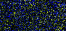
\includegraphics[width = .19\linewidth]{sb231_day_0}}
  \subcaptionbox{9 June\label{fig:day_24}}{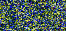
\includegraphics[width = .19\linewidth]{sb231_day_24}}
  \subcaptionbox{3 July\label{fig:day_48}}{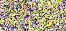
\includegraphics[width = .19\linewidth]{sb231_day_48}}
  \subcaptionbox{27 July\label{fig:day_72}}{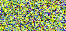
\includegraphics[width = .19\linewidth]{sb231_day_72}}
  \subcaptionbox{20 August\label{fig:day_96}}{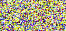
\includegraphics[width = .19\linewidth]{sb231_day_96}}
  \caption{Crop samples taken in 2016 over time, in Pauli decomposition}
  \label{fig:sample_images}
\end{figure}

The roadmap for the data analysis of these images is:
\begin{enumerate}
  \item Obtaining the geodesic purity index and scattering type angle of the data;
  \item Making a descriptive analysis of the data with histograms and boxplots;
  \item Fitting the data with models;
  \item Making separability tests.
\end{enumerate}

The geodesic purity index measures the distance between a target and the ideal depolarizer, which is characterized by the following Kennaugh matrix:
\[ \mathbf{K}_{\text{dep}} =
\begin{bmatrix}
1 & 0 & 0 & 0\\
0 & 0 & 0 & 0\\
0 & 0 & 0 & 0\\
0 & 0 & 0 & 0
\end{bmatrix}.
\]
The geodesic purity index is calculated as follows:
\begin{equation}
  P_{\text{GD}} = \left(\frac{3}{2}\text{GD}(\mathbf{K}, \mathbf{K}_{dep})\right)^2.
\end{equation}

\section{Data analysis}

\subsection{Geodesic Purity Index}

A first inspection of the purity indexes suggested that Beta distributions may be a good explanatory model.
The data look crammed in their original space, though.

After this initial qualitative analysis, we decided to transform the data applying the logarithmic function.
Fig.~\ref{fig:histograms_purity} shows the histograms and boxplots. 
The closeness to Gaussian distributions is remarkable.
The QQ-Plots shown in Fig.~\ref{fig:qqplots} provide more evidence of such good adherence.
Table~\ref{tab:pvalues_purities} provides the $p$-values of the Shapiro-Wilk test of goodness-of-fit to the Gaussian distribution.
There is no evidence, thus, to reject the hypothesis that the log-transformed purity data follows Gaussian distributions.

\begin{figure}[hbt]
  \centering
  \subcaptionbox{Histograms\label{fig:histograms_purity}}{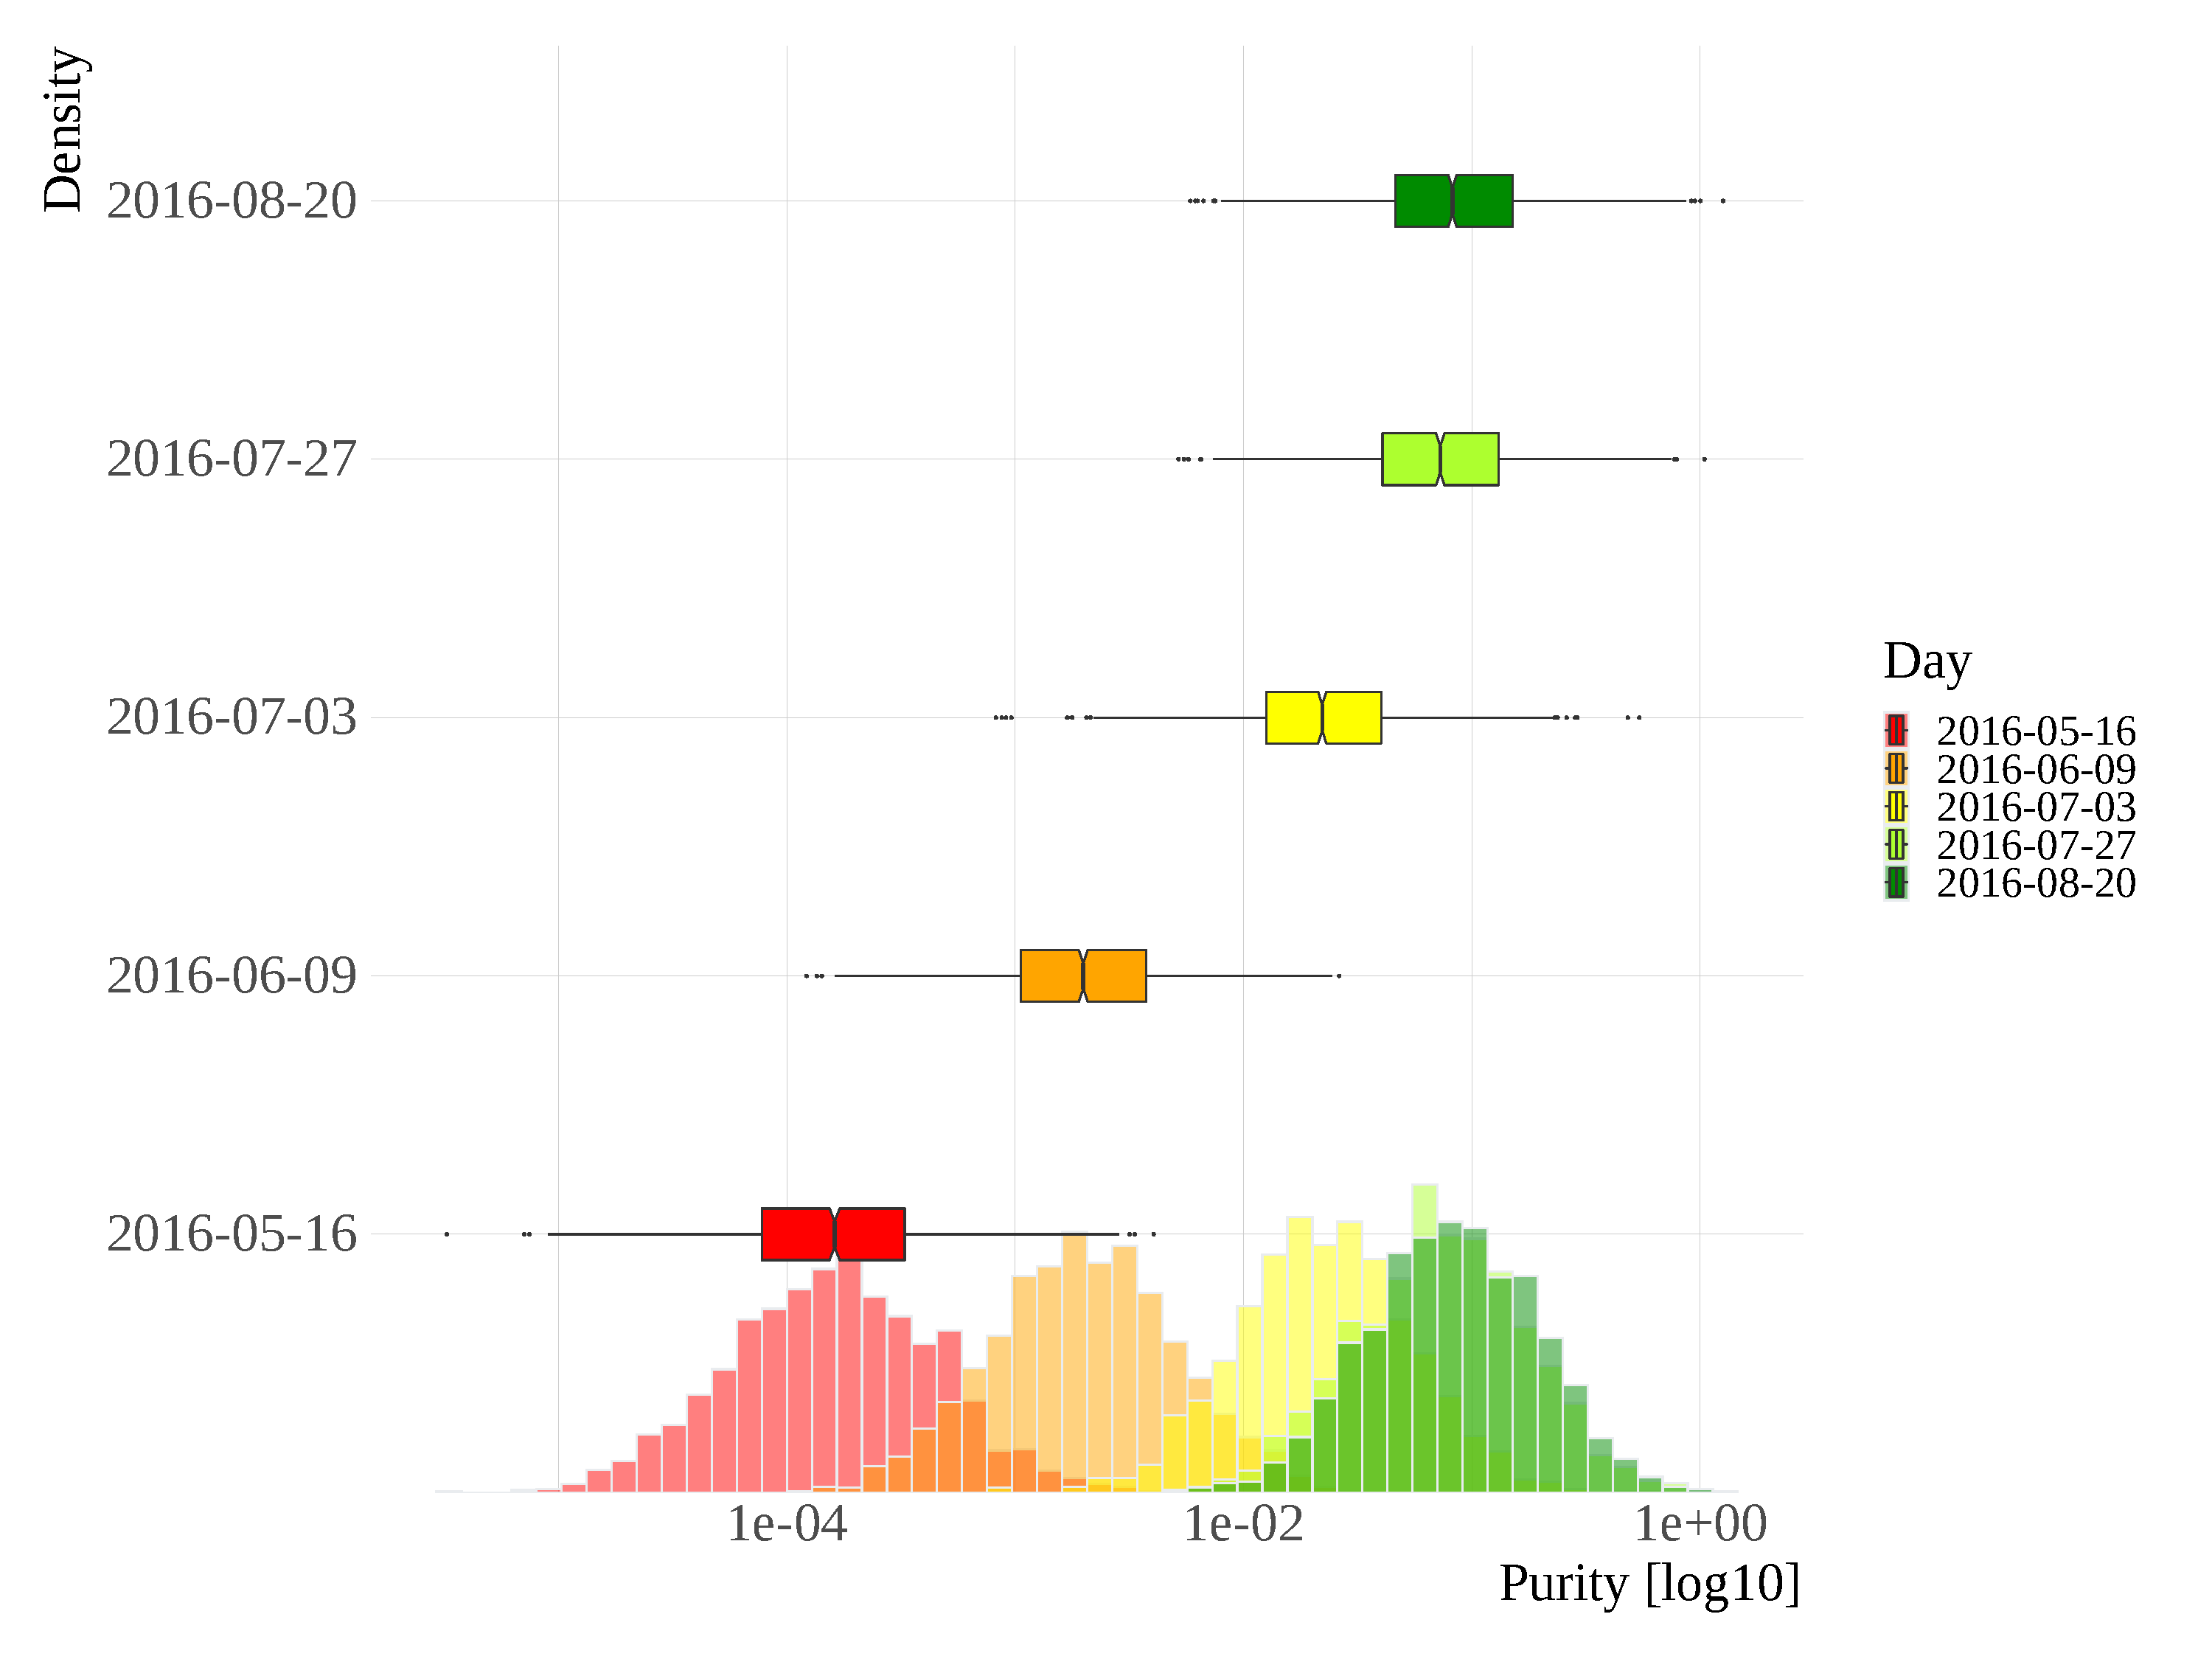
\includegraphics[width = .95\linewidth]{histograms}}
  \subcaptionbox{QQPlots\label{fig:qqplots}}{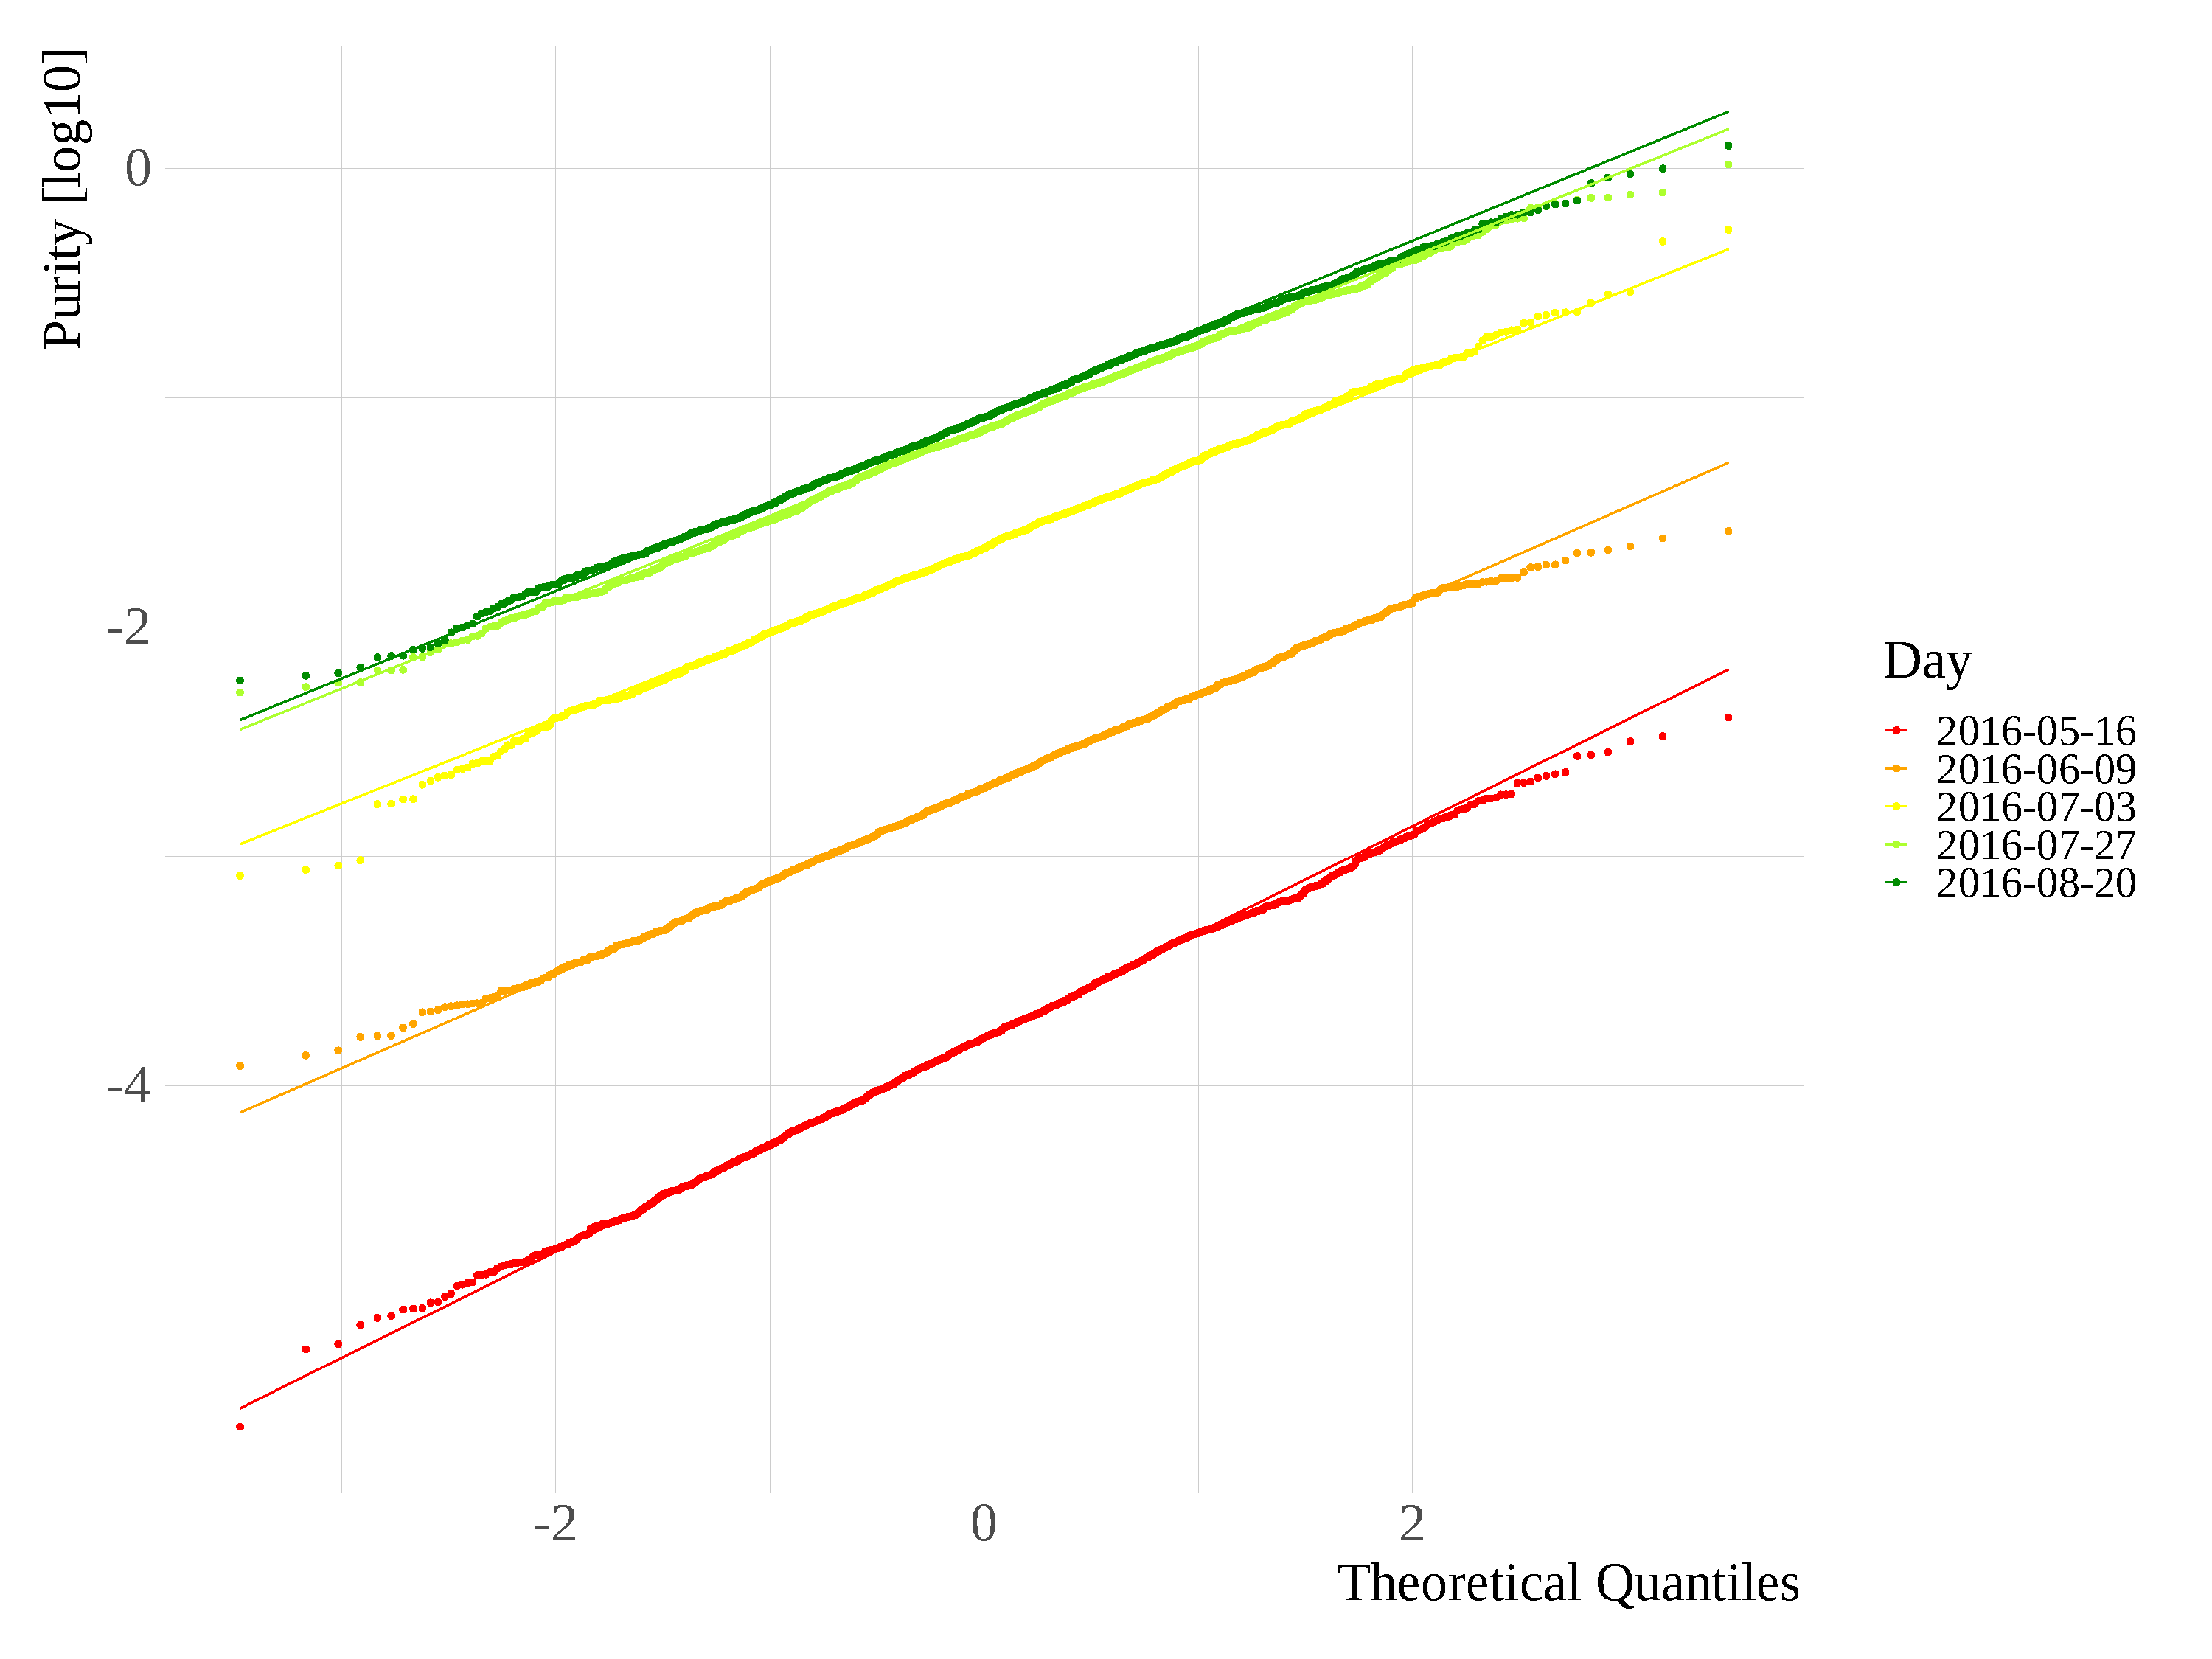
\includegraphics[width = .95\linewidth]{qqplots}}
  \caption{Descriptive analysis of the logarithm purity values for each image}
  \label{fig:desc_analysis}
\end{figure}

\begin{table}[hbt]
  \centering
  \caption{$p$-values from Shapiro-Wilk Test}
  \label{tab:pvalues_purities}
  \begin{tabular}{lrrrrr}
    \toprule
    \textbf{Day} & \textbf{16 May} & \textbf{09 June} & \textbf{03 July} & \textbf{27 July} & \textbf{20 Aug.}\\\midrule
    \textbf{$p$-value} & 0.4963 & 0.0650 & 0.3494 & 0.0585 & 0.3919\\
    \bottomrule
  \end{tabular}
\end{table}

\subsection{Geodesic Scattering Type Angle}

In this analysis, the geodesic distance to the trihedral - the normalized geodesic scattering type angle - was obtained from the samples. From these computed distances, those referring to pixels closer to the trihedral than to the other elementary scatterers (cylinder, dipole, dihedral, narrow dihedral, left helix, right helix, $-1/4$-wave, $+1/4$-wave) were selected.

From this selected distances per image, it was generated the histograms shown in the figure \ref{fig:histograms_alpha}. Through these graphs, one can suppose that these data obey a Beta distribution. To evaluate this assumption, the Komolgorov-Smirnov test was performed, whose $p$-values are in the table \ref{tab:pvalues_alpha} along with the sample size.

\begin{figure}[hbt]
\centering
\subcaptionbox{16 May}{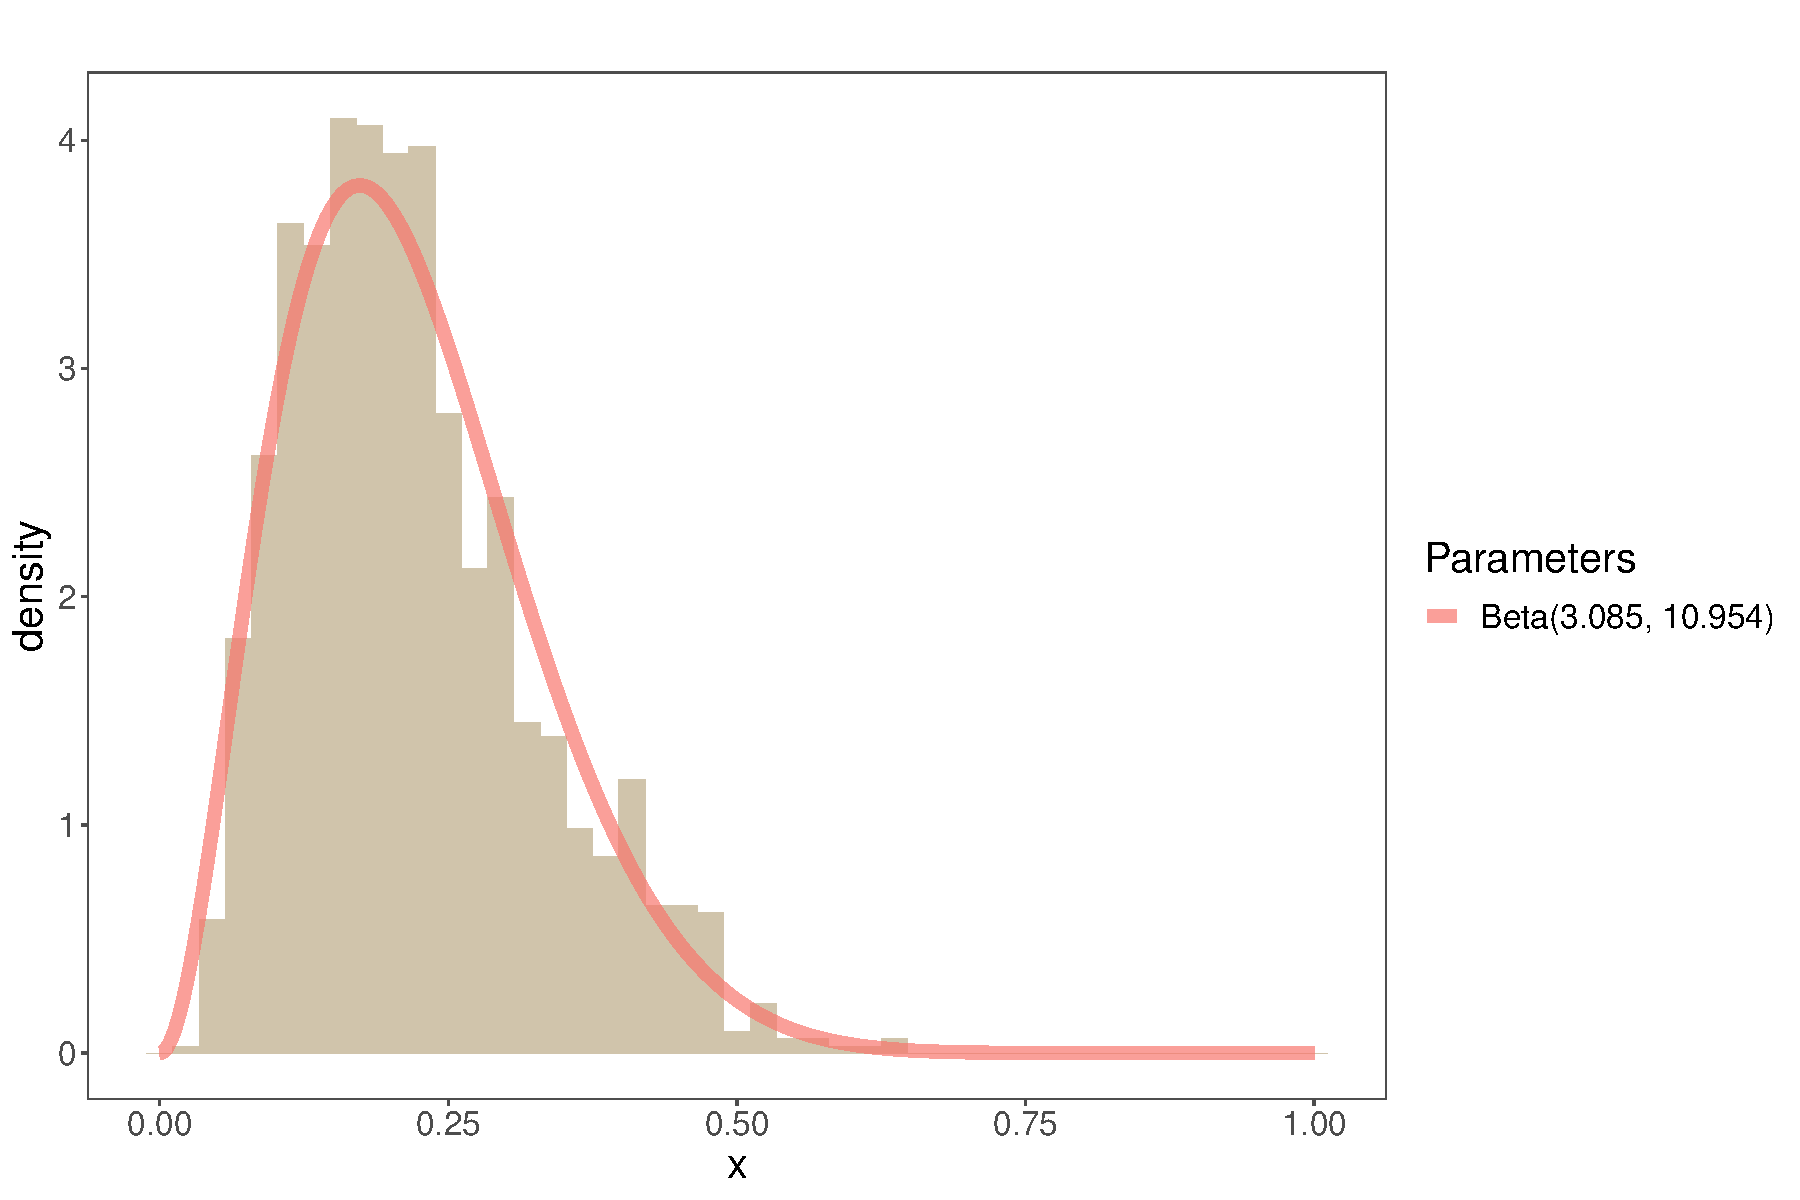
\includegraphics[width = .19\linewidth]{/Histograms/1th_observation/Soybeans_231/histogram_trihedral_1}}
\subcaptionbox{09 June}{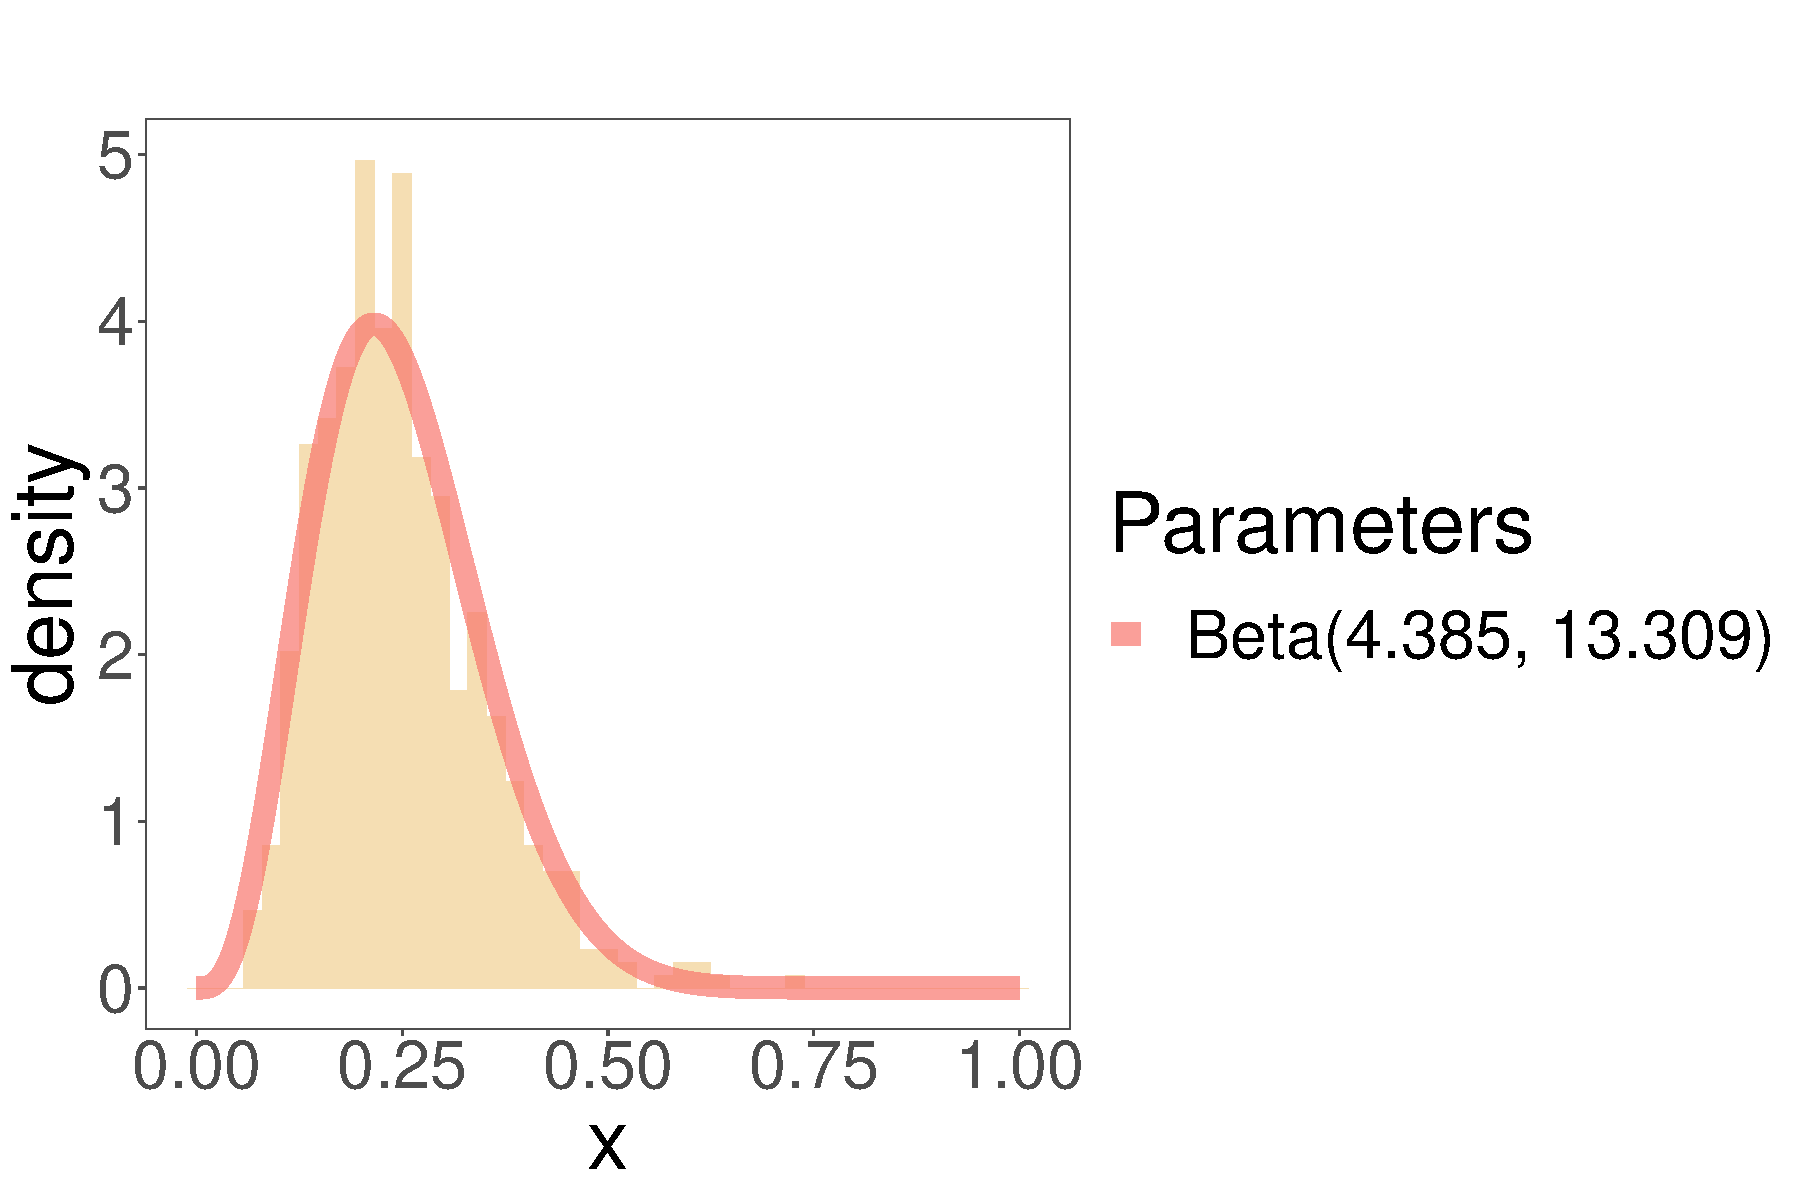
\includegraphics[width = .19\linewidth]{/Histograms/2th_observation/Soybeans_231/histogram_trihedral_2}}
\subcaptionbox{03 July}{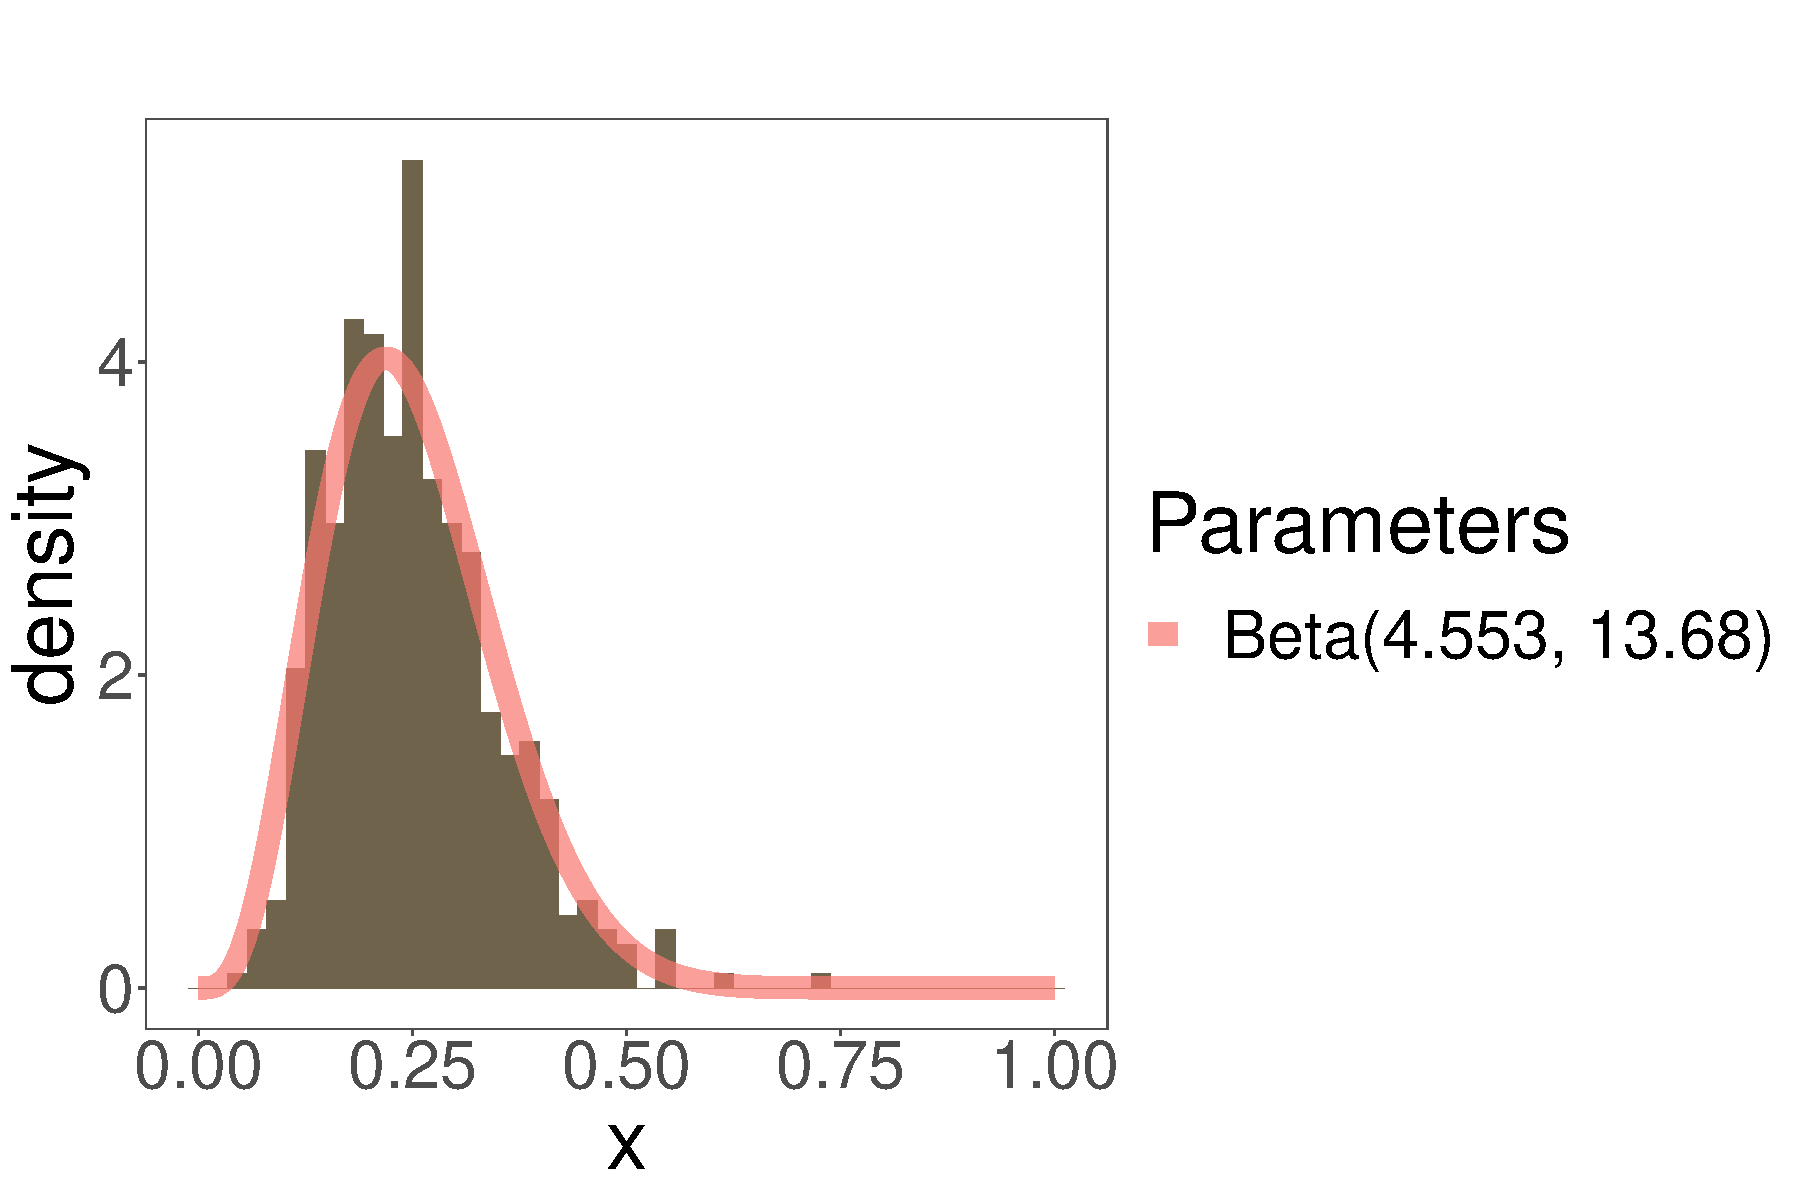
\includegraphics[width = .19\linewidth]{/Histograms/3th_observation/Soybeans_231/histogram_trihedral_3}}
\subcaptionbox{27 July}{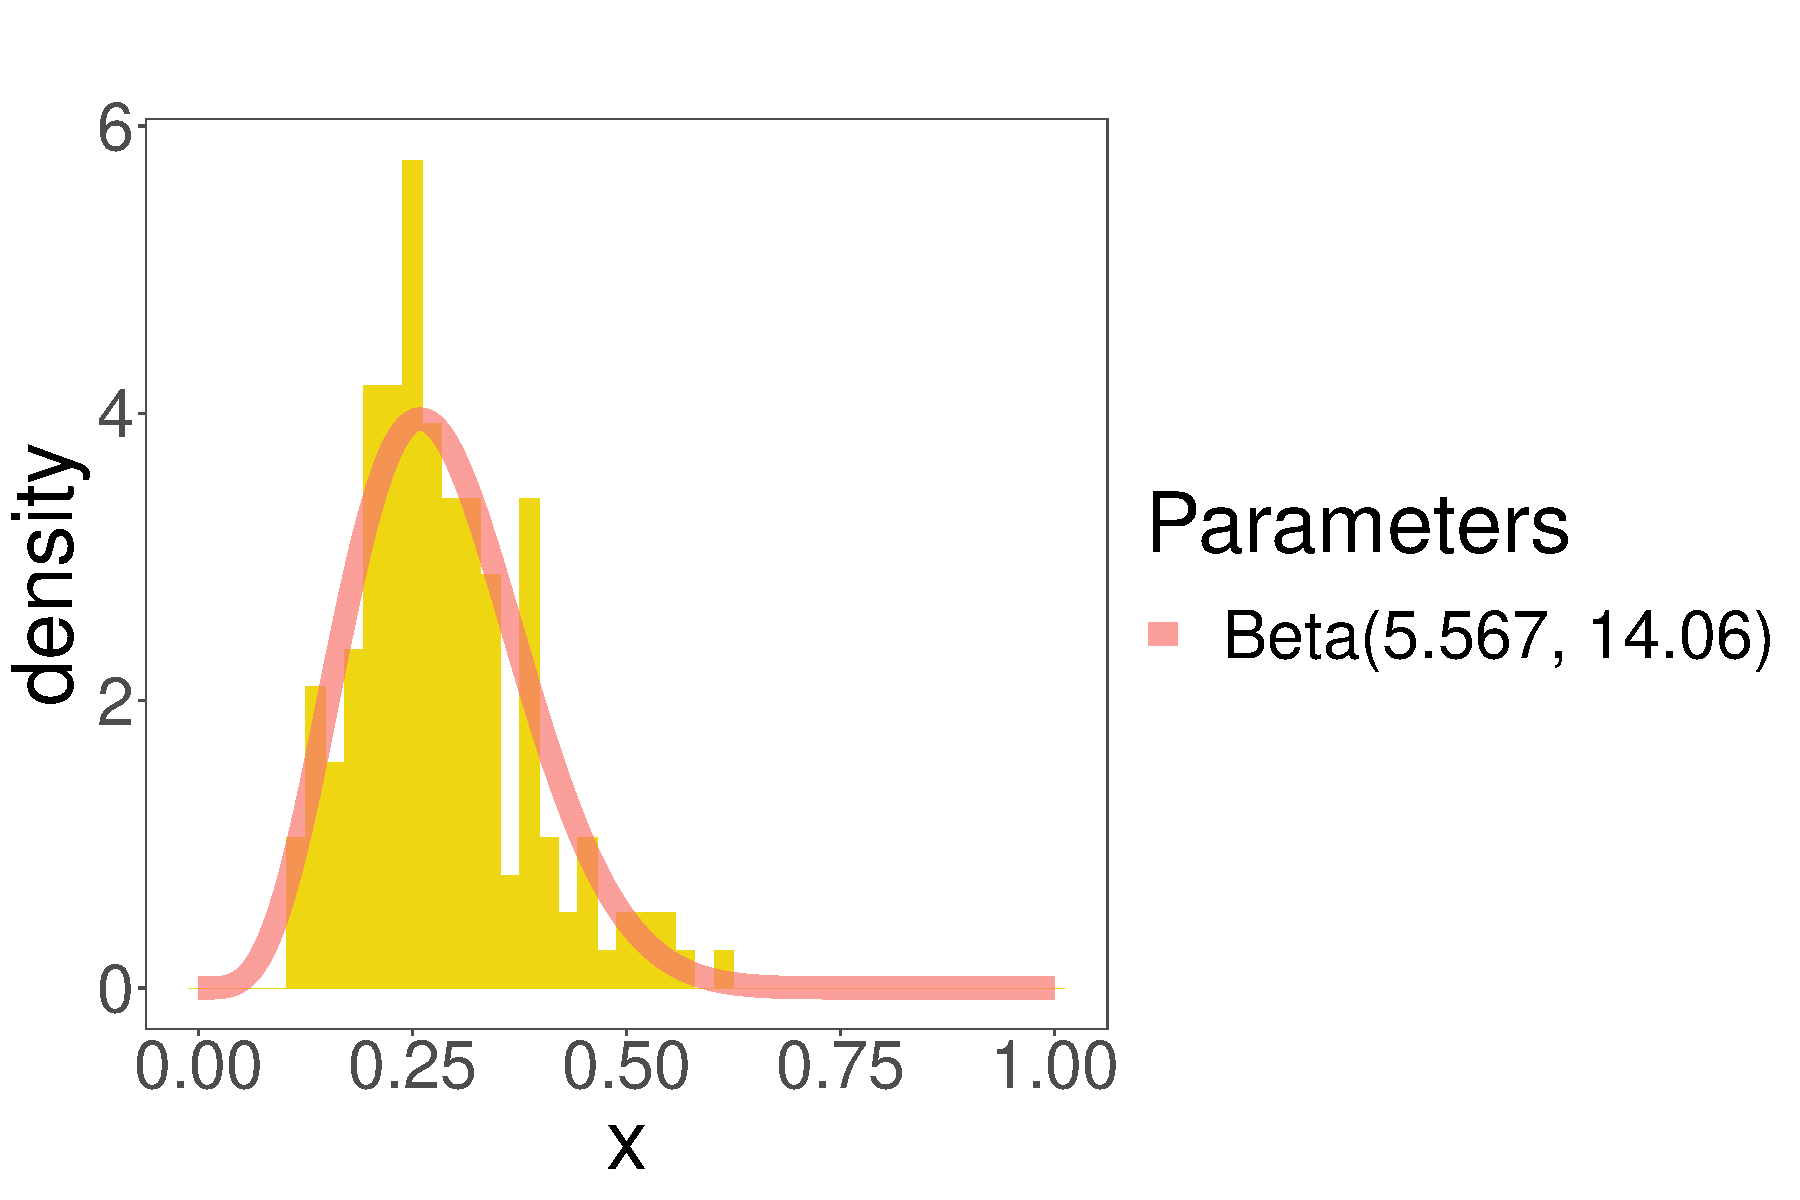
\includegraphics[width = .19\linewidth]{/Histograms/4th_observation/Soybeans_231/histogram_trihedral_4}}
\subcaptionbox{20 August}{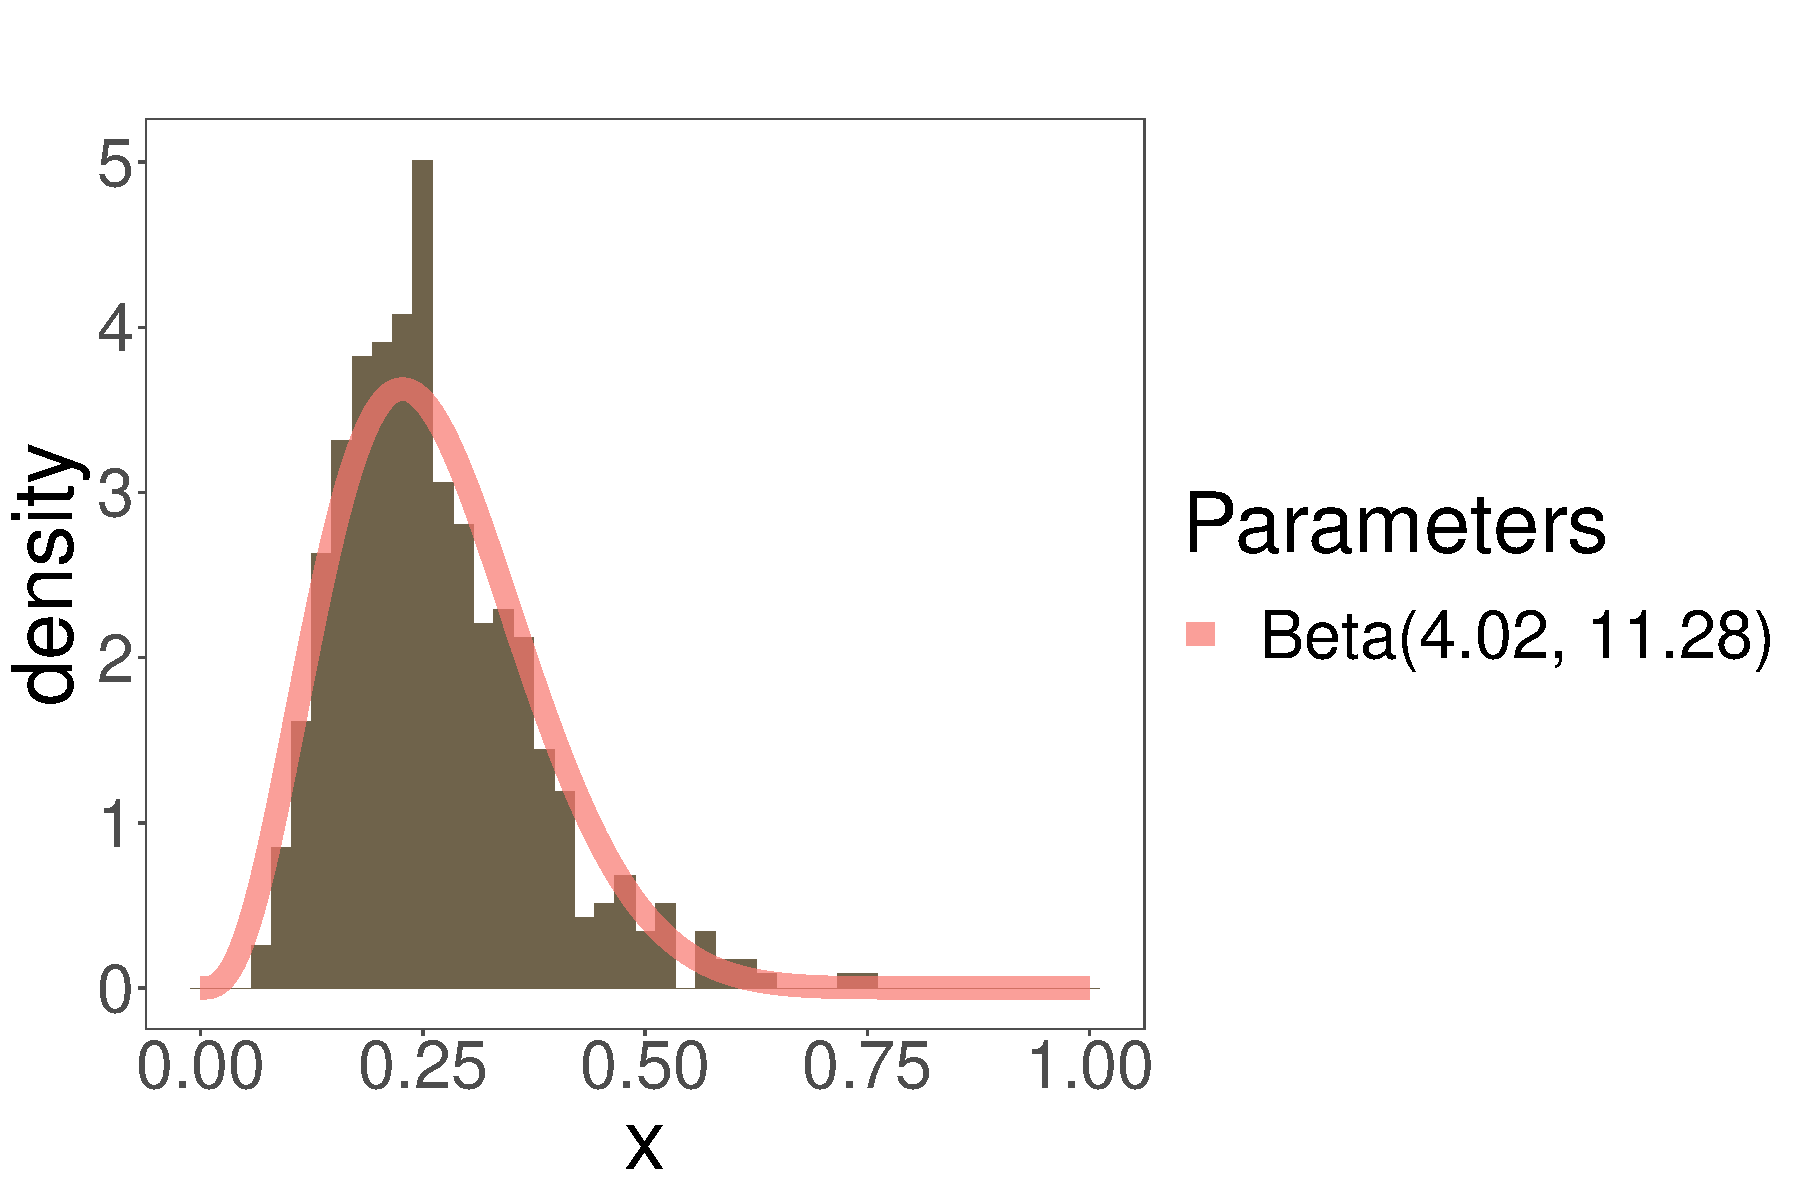
\includegraphics[width = .19\linewidth]{/Histograms/5th_observation/Soybeans_231/histogram_trihedral_5}}
\caption{Histograms of the geodesic distances between trihedral and the pixels of the samples most similar to trihedral}
\label{fig:histograms_alpha}
\end{figure}

\begin{table}[hbt]
  \centering
  \caption{$p$-values from Komolgorov-Smirnov Test}
  \label{tab:pvalues_alpha}
  \begin{tabular}{lrrrrr}
    \toprule
    \textbf{Day} & \textbf{16 May} & \textbf{09 June} & \textbf{03 July} & \textbf{27 July} & \textbf{20 Aug.}\\ 
                 & \textbf{2016} & \textbf{2016} & \textbf{2016} & \textbf{2016} & \textbf{2016}\\\midrule
    \textbf{Sample size} & 1285 & 656 & 449 & 615 & 508\\
    \textbf{$p$-value} & 0.7746 & 0.5734 & 0.3137 & 0.2392 & 0.4158\\
    \bottomrule
  \end{tabular}
\end{table}

Additionally, we performed a separability test based on the Hellinger distance between the original samples assuming the Beta distribution.
Table~\ref{tab:pvalues_sep_alpha} shows the $p$-values of the null hypothesis that each pair comes from the same law.
We observe that at level \num{0.05}, the only null hypothesis that cannot be rejected is that the data from the two last dates come from the same law.

\begin{table}[hbt]
  \footnotesize
  \centering
  \caption{$p$-values from Separability Test}
  \label{tab:pvalues_sep_alpha}
  \begin{tabular}{ccccc}
  \toprule
& \textbf{09 June} & \textbf{03 July} & \textbf{27 July} & \textbf{20 Aug.}\\ \midrule
  \textbf{16 May 2016}  & $7.467 \times 10^{-8}$ & $9.223 \times 10^{-12}$ & $5.159 \times 10^{-21}$ & $1.311 \times 10^{-24}$ \\
  \textbf{09 June 2016}  & --- & $2.640 \times 10^{-3}$ & $4.551 \times 10^{-4}$ & $1.757 \times 10^{-6}$ \\
  \textbf{03 July 2016}  & --- & --- & $4.318 \times 10^{-2}$ & $1.072 \times 10^{-2}$\\
  \textbf{27 July 2016}  & --- & --- & --- & $3.642 \times 10^{-1}$ \\
  \bottomrule
  \end{tabular}
\end{table}

\end{document}